%=====================%
\chapter{Neutron Activation for the \textsc{Majorana} Collaboration}
%=====================%
%-------------------------------------------------------------------%
\section{Introduction}
%-------------------------------------------------------------------%

Neutron activated samples of polytetrafluoroethylene (PTFE) and fluorinated ethylene propylene (FEP) tubing were \textgamma-assayed in the low background counting (LBC) lab at the Kimballton Underground Research Facility (KURF).  Presented in this report are activities from detected isotopes, many of which are neutron activation products of transition metals.

%-------------------------------------------------------------------%
\section{Sample Preparation}

Thinly sliced PTFE samples and small sections of FEP tubing were activated at various times from September 30, 2015, to October 2, 2015, at the PULSTAR high flux reactor at North Carolina State University (http://www.ne.ncsu.edu/nrp/pulstar.html).  Total time in the reactor over this period was 18 hours.  Samples of varying masses as shown in Figure 1.1 were placed in plastic vials and packaged for shipping to Virginia Tech (VT).  Ten vials containing 0.002-in thick PTFE samples were placed in a heat sealed plastic bag.  This plastic bag was placed inside of a resealable plastic bag and labeled accordingly.  Eight vials containing 0.005-in thick PTFE samples were placed in a heat sealed plastic bag along with the one vial containing FEP tubing.  The samples arrived at VT on October 7, 2015.  Environmental Health and Safety at VT received the samples and checked them for external contamination leakage.  None was found and all samples demonstrated no more than 0.2 mrem/hr of activity externally.  Samples were transported underground via the VT state-provided diesel truck to KURF on October 7, 2015.

% ------------  figure start  
\begin{figure}[htbp]
\centering
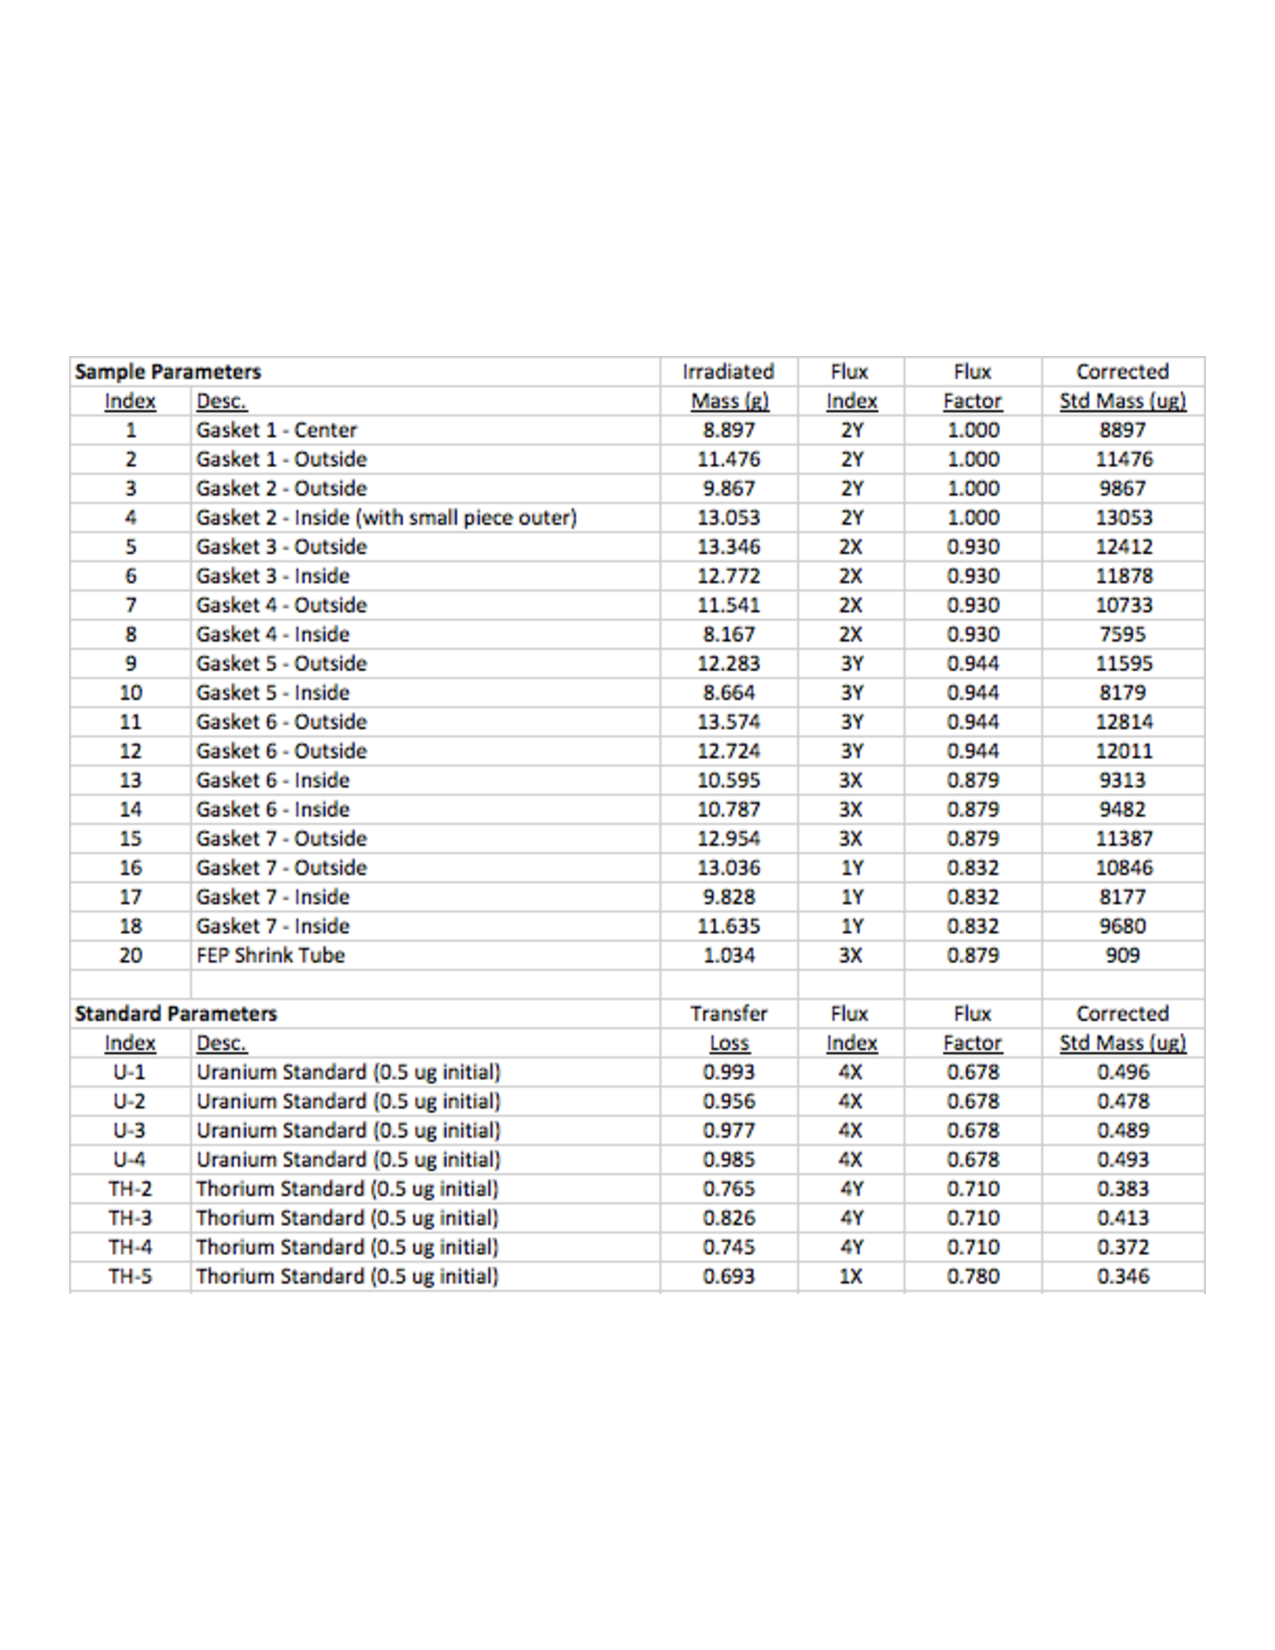
\includegraphics[width=1.0\textwidth]{/Users/JET/Dropbox/ENAP/Dissertation/2_neutronactivation/figures/naa_masschart.pdf}
\caption[%
Table of masses for neutron activated samples and standards.  
]{%
Table of masses for neutron activated samples and standards.  Information provided by Matthew Green at North Carolina State University.
\label{fig:mjd_cryostat}} 
\end{figure}
% ------------  figure end 

Samples were shipped along with vials containing irradiated aqueous solutions with trace uranium and thorium concentrations which were used to calibrate the spectra from the samples and to find the ratio between absolute U/Th levels in the samples and measured $\gamma$-ray activities.  The standards were packaged in sealed plastic bags as well as shown in Figure 1.2.

% ------------  figure start  
\begin{figure}[htbp]
\centering
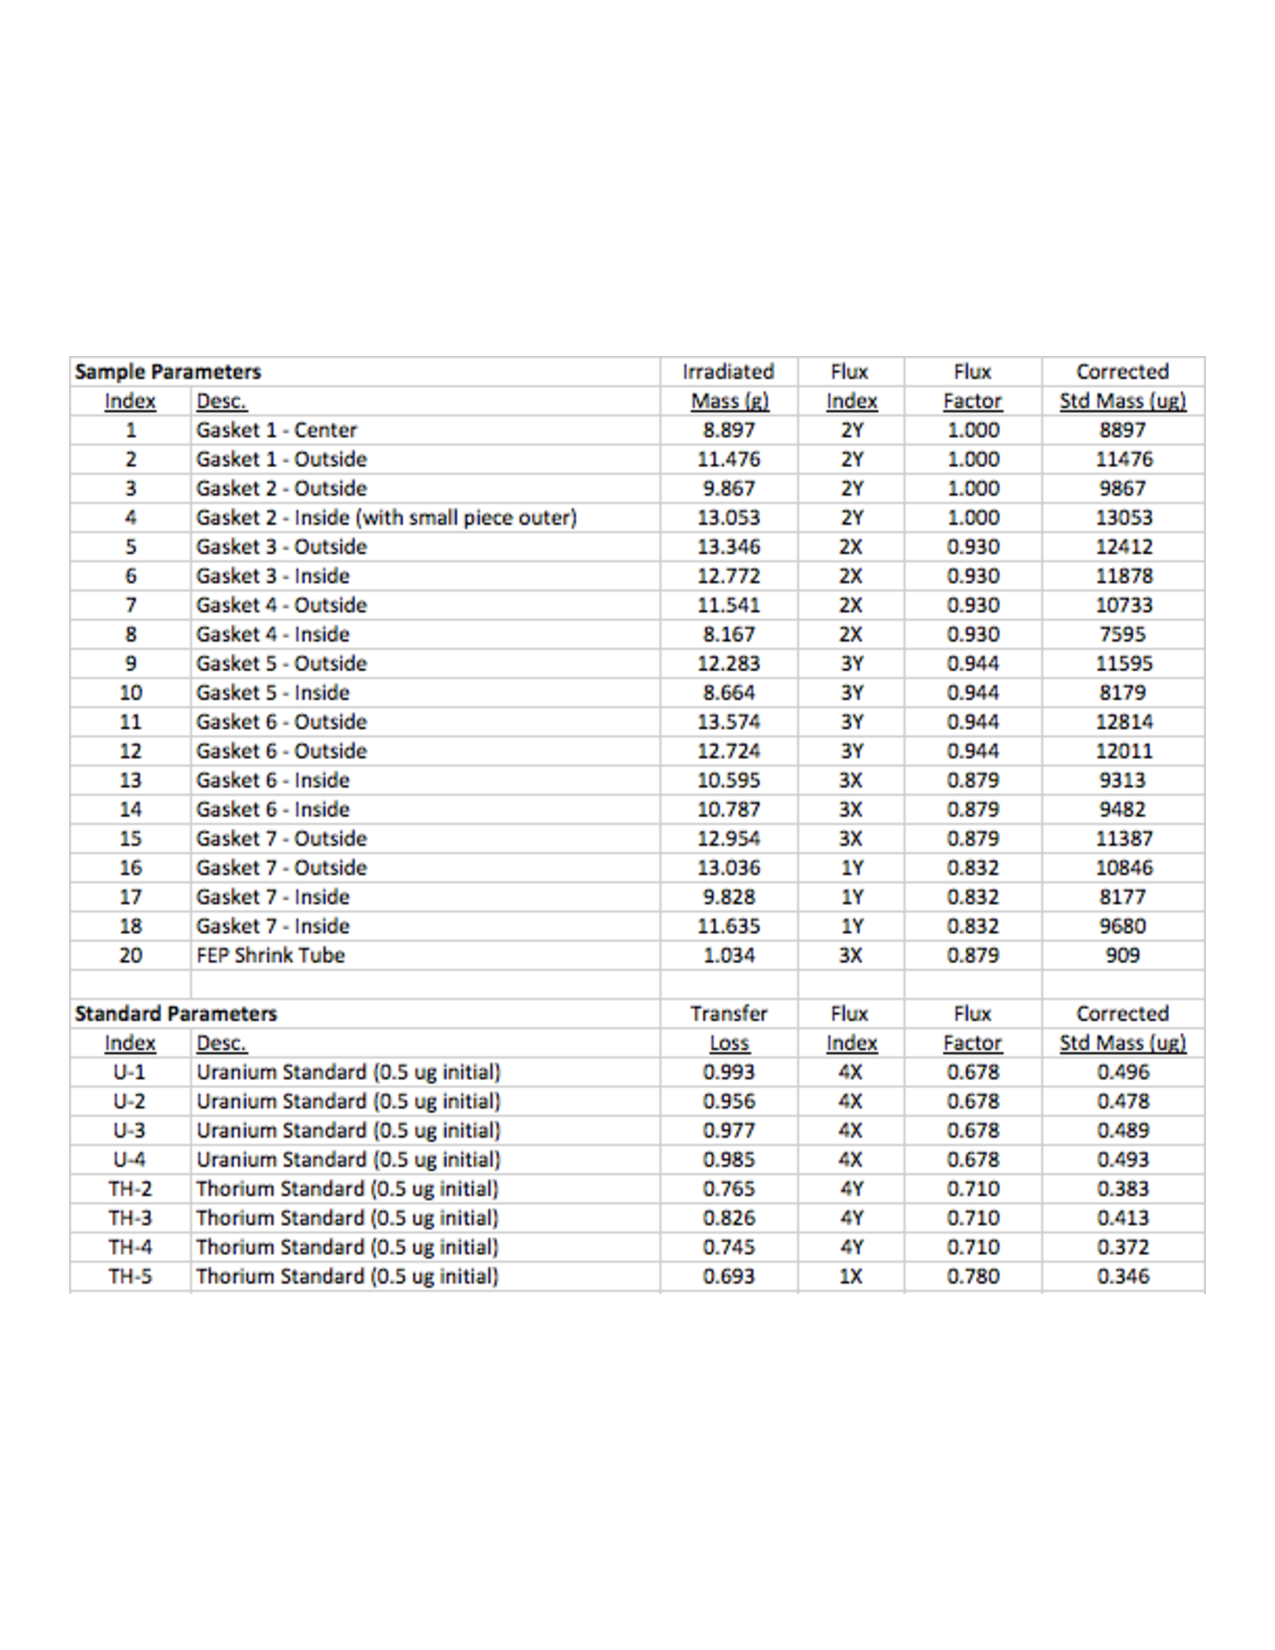
\includegraphics[width=0.7\textwidth]{/Users/JET/Dropbox/ENAP/Dissertation/2_neutronactivation/figures/naa_masschart.pdf}
\caption[%
Neutron activation sample packaging
]{%
Neutron activation sample packaging
\label{fig:mjd_cryostat}} 
\end{figure}
% ------------  figure end 

Upon arrival at the lab, a sample preparation station was arranged.  A table was placed outside of the detector lab with a plastic sheet on top.  Everything inside of the shipping container was treated as contaminated for safety purposes.  At all times, nitrile gloves were worn when handling anything that was inside the original shipping container or came in contact with something inside the shipping container.  Two Marinelli beakers were designated for use in the detectors with the samples.


%-------------------------------------------------------------------%
\section{Measurement}

Measurements were made using the two detectors at the UNC low-background counting facility at KURF.  The first detector,``\textsc{Melissa}," is a 1.1kg, 50\% RE (relative efficiency compared to NaI) Canberra LB (low-background) detector. \textsc{Melissa} is oriented vertically and is cooled using a dipstick cryostat. \textsc{Melissa}'s shield consists of 15 cm of Doe-run lead and 2.54 cm OFHC (oxygen-free high conductivity) copper. At the time of sampling, however, the top 30\% of the shield was unstacked due to previous detector maintenance.  The sample cavity is 38 cm $\times$ 38 cm $\times$ 38 cm.  The FWHM at 1.33 MeV is 1.70 keV, and the threshold is ~20 keV.   The other detector, ``VT-1," is a 0.956 kg, 35\% RE ORTEC LLB Series detector in a J-type configuration. VT-1's shield consists of a 10.1-cm ORTEC commercial lead shield and 0.3 cm of OFHC copper. The sample cavity  is cylindrical with dimensions 41 cm (height) $\times$ 28 cam (diameter).  VT-1 has a FWHM of 1.80 keV at 1.33 MeV and the threshold is ~20 keV. For more technical details regarding the facility and detector setup, see \cite{Fin10}.

Each standard vial was placed in one of the detectors for 20 minutes at a time.  For the first 20 minutes, the $^{238}$U standard was placed in \textsc{Melissa} and the $^{232}$Th standard was placed in VT-1.  For the second 20 minutes, the samples were each moved to the other detector.  The spectrum for the $^{238}$U standard in \textsc{Melissa} is shown in Figure 1.3 along with a magnification of the ROI in Figure 1.4  Figures 1.5 and 1.6 show the same spectra for the $^{232}$Th standard.  After the standards were measured, the 0.002-in PTFE samples were placed in \textsc{Melissa} and the FEP tubing samples were placed in VT-1 for assay.  Emphasis was placed on these two samples at the request of the \textsc{Majorana} project engineer.  

% ------------  figure start  
\begin{figure}[htbp]
\centering
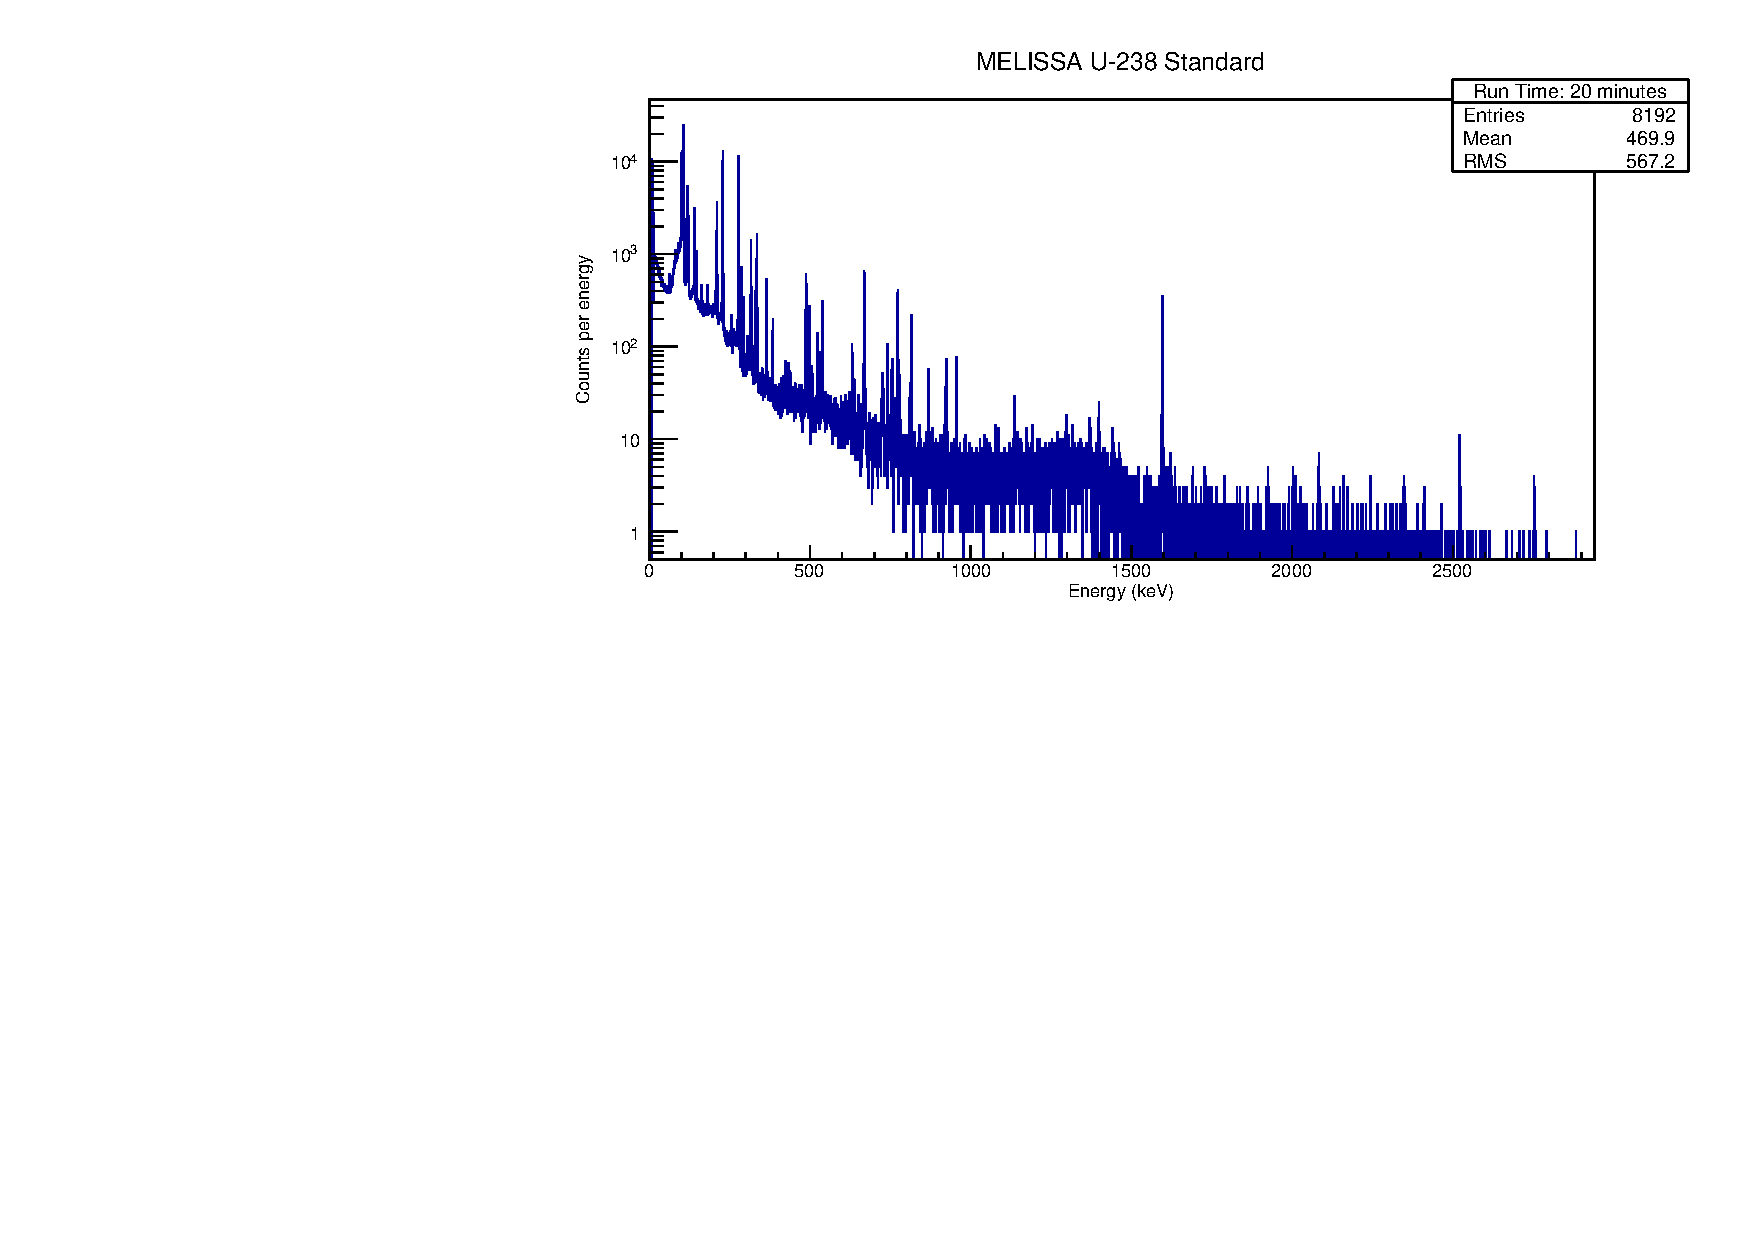
\includegraphics[width=1.0\textwidth]{/Users/JET/Dropbox/ENAP/Dissertation/2_neutronactivation/figures/MEL_run_412-412.pdf}
\caption[%
$^{238}$U standard spectrum in \textsc{Melissa}
]{%
$^{238}$U standard spectrum in \textsc{Melissa}
\label{fig:mjd_cryostat}} 
\end{figure}
% ------------  figure end 

% ------------  figure start  
\begin{figure}[htbp]
\centering
\includegraphics[width=1.0\textwidth]{/Users/JET/Dropbox/ENAP/Dissertation/2_neutronactivation/figures/MEL_run_412-412_zoom.pdf}
\caption[%
$^{238}$U standard spectrum in \textsc{Melissa} showing peak at 106 keV
]{%
$^{238}$U standard spectrum in \textsc{Melissa} showing peak at 106 keV
\label{fig:mjd_cryostat}} 
\end{figure}
% ------------  figure end 

% ------------  figure start  
\begin{figure}[htbp]
\centering
\includegraphics[width=1.0\textwidth]{/Users/JET/Dropbox/ENAP/Dissertation/2_neutronactivation/figures/MEL_run_413-413.pdf}
\caption[%
$^{238}$Th standard spectrum in \textsc{Melissa}
]{%
$^{238}$Th standard spectrum in \textsc{Melissa}
\label{fig:mjd_cryostat}} 
\end{figure}
% ------------  figure end 

% ------------  figure start  
\begin{figure}[htbp]
\centering
\includegraphics[width=1.0\textwidth]{/Users/JET/Dropbox/ENAP/Dissertation/2_neutronactivation/figures/MEL_run_413-413_zoom.pdf}
\caption[%
$^{238}$Th standard spectrum in \textsc{Melissa} showing peak at 312 keV
]{%
$^{238}$Th standard spectrum in \textsc{Melissa} showing peak at 312 keV
\label{fig:mjd_cryostat}} 
\end{figure}
% ------------  figure end 


Once the standards were measured and the spectra were reviewed, the samples were placed in the detectors.  The ten vials containing 0.002-in thick slices of PTFE were placed in a Marinelli beaker inside \textsc{Melissa}.  The samples were oriented as shown in Figure 1.7.  The vial containing the FEP tubing was placed in a Marinelli beaker inside of VT-1.  Both detectors were sealed and the data collection was allowed to run for 30 hours.  All analysis was based on this 30-hour period.

%------------------------------------------------------------------%
\section{Analysis}

%For analysis, a sample spectrum is compared to the spectra for both standards.  Using a library of common gamma lines seen in neutron activation, we then search for peaks that can be used to measure the activity of the sample.  For the best results, well-separated peaks with the highest intensities are used.  For low statistics situations such as this case, the ROI is determined using the detector energy resolution, $\sigma_{res}$.  

%Subtraction of the continuum is then done by defining two regions, one $10\sigma$ to the left and the other $10\sigma$ to the right of the peak, averaging the sum of the counts in the two regions, and then subtracting from the total integrated peak area.  If another peak is between $5\sigma$ and $15\sigma$ to the left or right, only the region excluding the extra peak is used for averaging.  An adjustment factor is multiplied to the integrated cotinuum area to give an effective range of $10\sigma$ for either side.  If another peak is within $5\sigma$, then only one side of the peak is integrated for continuum subtraction.

The number of counts in ROI for the standards are found by subtracting the background from the peak in the ROI.  The net peak area is found by subtracting the peak area of a background peak from the corresponding standard peak.  The background in this case was found by fitting a linear function to a region extending $\pm$3$\sigma_{res}$ from the centroid of the peak in the standard.  

The activities of a specific peaks in the standards are then given by:

\begin{eqnarray}
A_{\gamma s} = \frac{N}{\epsilon_\gamma m t}
\end{eqnarray}

\noindent where $N$ is the net peak area at the energy observed, $\epsilon_\gamma$ is the estimated peak efficiency, $t$ is the assay live time, and $m$ is the mass of the standard.  This activity was then used to find the initial activity for the isotopes of interest with:

\begin{eqnarray}
A_{os} &=&A_{\gamma s}e^{\lambda \bar{t}}
\end{eqnarray}

\noindent where $A_{os}$ is the initial activation activity, $A_{\gamma s}$ is the net peak area of the irradiated standards at known energies, $\bar{t}$ is the average time since activation, and $\lambda$ is the decay constant for that isotope.  

The same energies were then observed from samples' spectra.  The ROI was defined as the same $\pm$3$\sigma_{res}$ regions used to analyze the standards.  If no statistically significant peak is present, an upper limit can be placed on the activity in a sample.  The signal in an energy bin is then required to be less than or equal to the upper limit, 90\% C.L. - $1.65\sigma$ ($\sigma$ here is just the square root of the recorded counts).  We can convert this limit on the counts to a limit on the mass fraction of the isotope using the measured activities in the activated standards.  This is given by:

\begin{eqnarray}
Mass Fraction Limit&=&1.65 \frac{\sqrt{A_p}}{t  m  \epsilon_\gamma} \frac{1}{A_{os}} e^{\lambda \bar{t}}
\end{eqnarray}

where $A_p$ is the activity in the ROI for the sample, $t$ is the assay live time of the sample, $m$ is the mass of the sample, $\epsilon_\gamma$ is the estimated efficiency, $A_{os}$ is the initial activity of the standard, $\bar{t}$ is the average time since activation, and $\lambda$ is the decay constant.  This mass fraction is the activity limit of the calculated original activity of the sample in part per trillion (ppt).



%\begin{eqnarray}


%Peak efficiencies are determined using a detailed Monte Carlo simulation in \textsc{Geant}4.  Once a detailed sample geometry has been coded into the simulation, it is doped uniformly with isotopes of interest,  usually from the $^{238}$U, $^{232}$Th, and $^{40}$K decay chains, along with any others that may be present in the sample, e.g. $^{60}$C.  The primary $\gamma$-rays from these decays are tracked from the emission of the source to absorption in the detector active region.   The main advantages to using a pure Monte Carlo simulation is that self-attenuation in the sample is accounted for and the are no limitations on source or detector configurations.

%The energy deposits in the simulated spectrum are convolved with the finite energy resolution of the detector.  The resolution factor, $\sigma_{res}$, has been measured as a function of $\gamma$-ray energy ($E_{keV}$) from 303-1836 keV using radioactive point sources.  Using the following equation from \cite{Fin10}, these data were fit to

%\begin{eqnarray}
%\sigma_{res} &=& \sqrt{a^2 + b^2 E_{keV} + c^2 E^{2}_{keV}}
%\end{eqnarray}

%The net peak area in the simulated spectrum is determined by fitting the peak of interest with a Gaussian and subtracting a linear background.  A correction term must also be included to account for systematic error in the Monte Carlo.  For a sample in Melissa located near the top of the detector, f = $1.04\pm0.06$ \cite{Fin10}.  The absolute peak efficiency, including branching ratios, can then be determined from 

%\begin{eqnarray}
%\sigma_\gamma &=& f\frac{N}{N_o}
%\end{eqnarray}

%\noindent where $N_o$ is the number of events simulated.

%---------------------------------------------------------------------------%
\section{Results}

A list of $\gamma$-active isotopes found in the spectra is given for both the 0.002-in thick PTFE and the FEP tubing.  All isotopes found were products of neutron activation.  The isotopes of interest for this assay were products of the neutron activation of $^{238}$U and $^{232}$Th impurities in the samples, specifically the peaks at 106 keV for $^{239}$Np and 311 keV
for $^{233}$Pa respectively.  No statistically significant peaks were found at either energy.  Calculated initial activity limits of $^{238}$U and $^{232}$Th in the 0.002-in PTFE samples were 5.2 ppt and 3.5 ppt respectively.  The same limits in the FEP tubing sample were 9.4 ppt and 6.3 ppt respectively.  A list of additional isotopes identified in the samples is shown in Table 1.1.


%\section{Additional Detected Isotopes}

%\noindent $^{51}$C (t$_{1/2}$ = 28d): Line at 320 keV.

%\noindent $^{82}$Br (t$_{1/2}$ = 35h): Lines at 554, 620, 698, 764, 776, 827, 1043, 1316, and 1474 keV.

%\noindent $^{110}$Ag (t$_{1/2}$ = 250d): Lines at 657, 707, 884, 937, and 1383 keV.

%\noindent $^{60}$Co (t$_{1/2}$ = 1925d): Lines at 1173 and 1333 keV.

%\noindent $^{54}$Mn (t$_{1/2}$ = 312d): Line at 835 keV.

%\noindent $^{58}$Co (t$_{1/2}$ = 71d): Line at 810 keV.

%\noindent $^{59}$Fe (t$_{1/2}$ = 44d): Lines at 1098 and 1291 keV.

%\noindent $^{65}$Zn (t$_{1/2}$ = 1115): Line at 244d keV.

%\noindent $^{22}$Na (t$_{1/2}$ = 3y): Line at 1273 keV.

%\noindent $^{24}$Na (t$_{1/2}$ = 15h): Lines at 1368 and 2751 keV.

%\noindent $^{124}$Sb (t$_{1/2}$ = 60d): Lines at 603 and 1690 keV.

%\noindent $^{40}$K (t$_{1/2}$ = 1.25$\times$10$^9$y): Line at 1460 keV.

%\noindent $^{123}$Sn (t$_{1/2}$ = 129d): Line at 159 keV.

\begin{table}
	\centering	
	\begin{tabular} { | l | l | l |}
	\hline
	\textbf{Isotope} & \textbf{Half-life} & \textbf{Lines observed (keV)} \\ \hline
	$^{51}$C & 28 days &  320 \\ \hline
	$^{82}$Br & 35 hours & 554, 620, 698, 764, 776, 827, 1043, 1316, 1474  \\ \hline
	$^{110}$Ag & 250 days & 657, 707, 884, 937, 1383 \\ \hline
	$^{60}$Co & 1925 days & 1173, 1333 \\ \hline
	$^{54}$Mn & 312 days & 835 \\ \hline
	$^{58}$Co & 71 days & 810 \\ \hline
	$^{59}$Fe & 44 days & 1098, 1291 \\ \hline
	$^{65}$Zn & 244 days & 1115 \\ \hline
	$^{22}$Na & 3 years & 1273 \\ \hline
	$^{24}$Na & 15 hours & 1368, 2751 \\ \hline
	$^{124}$Sb & 60 days & 603, 1690 \\ \hline
	$^{40}$K & 1.25$\times$10$^9$ years & 1460 \\ \hline
	$^{123}$Sn & 129 days & 159 \\ \hline
	\end{tabular}
	\caption{List of additional isotopes detected in the samples}
	\label{List of additional isotopes detected in the samples}
\end{table}




%\begin{eqnarray}
%^{238}U + n &\to& ^{239}U^*
%\end{eqnarray}

%\begin{eqnarray}
%^{239}U^* &\to& ^{239}Np + e^{-}  + \bar{\nu}_e
%\end{eqnarray}







